\documentclass[../review_3.tex]{subfiles}
\graphicspath{{\subfix{../img/}}}
\begin{document}

\chapter{Feinentwurf}\thispagestyle{fancy}
In diesem Kapitel zum Feinentwurf wird der im vorherigen Kapitel beschriebene Grobentwurf verfeinert. Dabei wird für jedes Paket präzise erklärt, auf welche Art und Weise die entsprechende Komponente realisiert werden soll, sodass diese dann direkt implementiert werden kann. Zudem werden mithilfe von Aktivitätsdiagrammen die Kernfunktionen des jeweiligen Pakets übersichtlich und grafisch dargestellt.

\section{ConfigurationManagement}
Die folgenden Klassen sind im Paket \texttt{ConfigurationManagement} enthalten.

\subsection{Configurator}
Für die Software gibt es die Konfigurationsdatei \texttt{config.JSON}, welche innerhalb dieser Klasse eingelesen wird und diese Informationen global zur Verfügung stellt. Von dieser Klasse, dem \texttt{Configurator}, soll es im ganzen Programmablauf nur ein Objekt geben, damit keine Inkonsistenzen entstehen.
\begin{figure}[H]
    \centering
    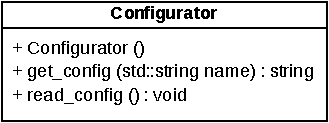
\includegraphics[width=0.4\linewidth]{img/Configurator.pdf}
    \caption{Klassendiagramm: \texttt{Configurator}}
    \label{Class_Configurator}
\end{figure}
Aufgrund dieser Anforderungen kann ein spezielles Entwurfsmuster verwendet werden: Das Singleton. Das Singleton ist ein Erzeugungsmuster, welches automatisch dafür sorgt, dass nur eine Instanz des \texttt{Configurator} existieren kann, und es stellt ähnlich globalen Variablen Informationen global dar. Der Vorteil des Singleton besteht darin, dass das Singleton nur dann verwendet wird, wenn es wirklich benötigt wird. Die Klasse \texttt{Configurator} hat nur einen privaten Konstruktor, welcher in der zum Singleton gehörigen Methode der Instanziierung verwendet wird. In der ersten Verwendung des \texttt{Configurators} wird die Methode \texttt{read\_config()} zur Einlesung der Daten ausgeführt. Falls die Konfigurationsdatei nicht auffindbar ist, so wird eine Exception geworfen, da die Software ohne diese nicht ablaufen kann. Die ausgelesenen Daten werden dann in einem privaten JSON-Objekt hinterlegt. Hierzu wird \texttt{nlohmann::JSON} verwendet. Die Informationen der JSON-Datei werden über eine Schnittstelle \texttt{get\_config(Datentyp)} anderen Klassen zur Verfügung gestellt, wobei es unterschiedliche Methoden je nach Datentyp gibt. Der explizite Aufruf des Auslesens erfolgt über die Methode \texttt{instance()}, mithilfe jener ein Zeiger auf das \texttt{Configurator}-Objekt zurückgegeben wird.

\subsection{Initializer}
Die Klasse \texttt{Initializer} dient dazu, dass grundlegende Initialisierungen für DPDK vorgenommen werden. Hierzu existiert die Methode \texttt{init\_dpdk(int argc, char** argv)}.

\subsection{Thread}
Die Klasse \texttt{Thread} dient dazu, parallele Threads erzeugen zu können, welche dann die gesamte Paketbehandlung des Systems durchlaufen. Hierzu werden jedem Thread zwei \texttt{PacketContainer} übergeben. Ein \texttt{PacketContainer} dient zum Annehmen von Paketen, welche von außerhalb des Netzwerkes in das Netzwerk kommen. Der andere \texttt{PacketContainer} dient analog zum Annehmen von Paketen, welche von innerhalb des Netzwerkes nach außen sollen. Die \texttt{run()}-Methode der \texttt{Thread}-Klasse hat die Aufgabe, dass eine bestimmte Anzahl an Paketen geholt wird, und zwar mittels der Methode \texttt{poll\_packets(int number)}. Dies gilt für beide \texttt{PacketContainer}. Nachdem die Pakete behandelt wurden, was innerhalb dieses Pollings vorgenommen wird, werden die restlichen Pakete mittels \texttt{send\_packets()} in die jeweilige Richtung weitergeschickt.

\section{PacketDissection}
Die Aufgabe der \texttt{PacketDissection} ist es, Informationen über die zu untersuchenden Pakete bereitzustellen. Zudem wird die Kommunikation des \texttt{NicManagements} über die \texttt{PacketDissection} geleitet.

In Diagramm \ref{Sequenzdiagramm_PacketDissection} wird das Polling von Paketen unter Benutzung des \texttt{PacketContainers} dargestellt. Der \texttt{PacketContainer} fungiert hierbei als zentrales Element zur Ablaufsteuerung.

\begin{figure}
    \centering
    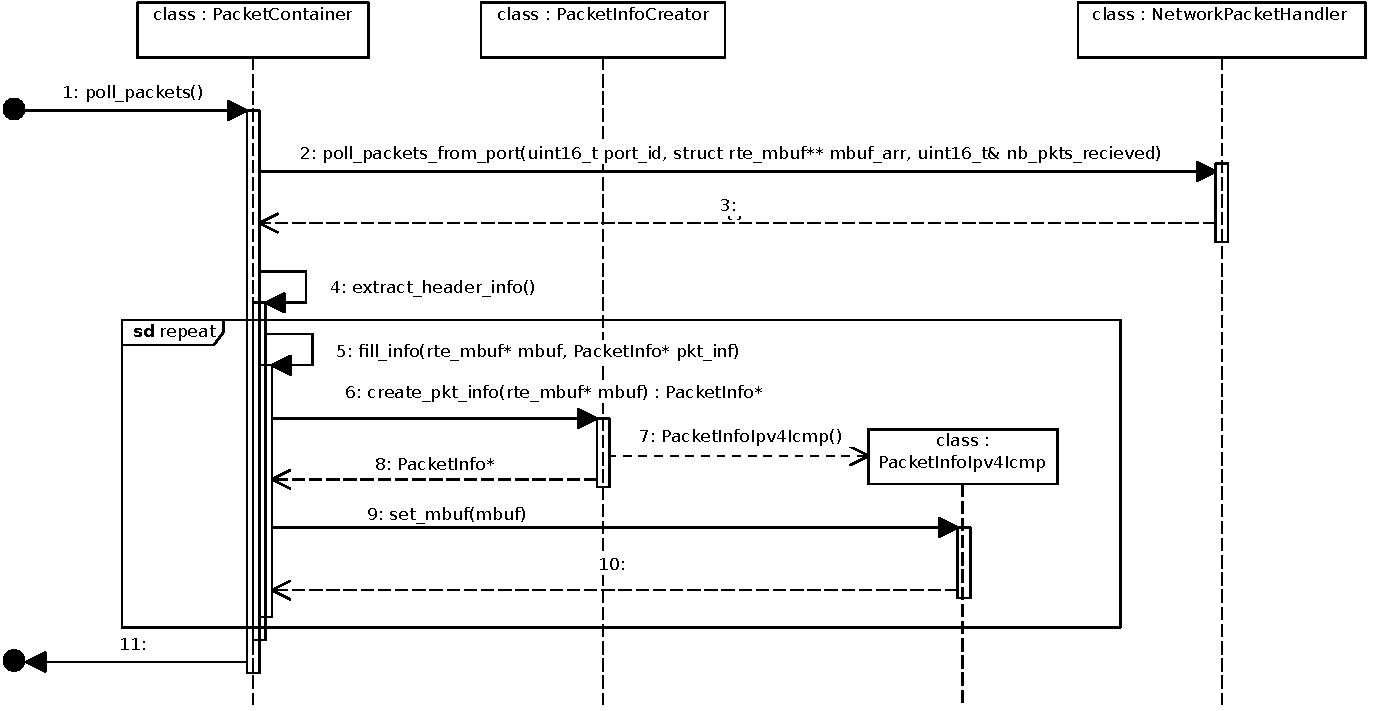
\includegraphics[width=\linewidth]{img/SequenceDiagramPacketDissection2.pdf}
    \caption{Sequenzdiagramm zum Polling von Paketen über den \texttt{PacketContainer}}
    \label{Sequenzdiagramm_PacketDissection}
\end{figure}

\subsection{PacketContainer}
DPDK liefert beim Pollen von Paketen ein Array von Pointern auf sogenannte \texttt{mbuf}-Strukturen. Auch beim Senden muss dem Framework ein solches Array übergeben werden, denn die \texttt{mbuf}-Strukturen repräsentieren Pakete innerhalb von DPDK. Um nur die \texttt{PacketInfo}-Objekte durch das Programm zu reichen, wäre das Array von \texttt{mbuf}-Strukturen zu durchlaufen und die Pointer jeweils in die \texttt{PacketInfo}-Objekte zu schreiben. Ein \texttt{mbuf}(-Paket) gehört dabei genau einer \texttt{PacketInfo}. Wenn am Ende der Pipeline Pakete gesendet werden, müssten die Pointer der \texttt{mbuf}-Strukturen den \texttt{PacketInfo}-Objekten wieder entnommen und in ein Array geschrieben werden. Dies ist überflüssiger Aufwand, da es möglich ist, das empfangene \texttt{mbuf}-Array beizubehalten. Dies setzt der \texttt{PacketContainer} um.

\begin{figure}
    \centering
    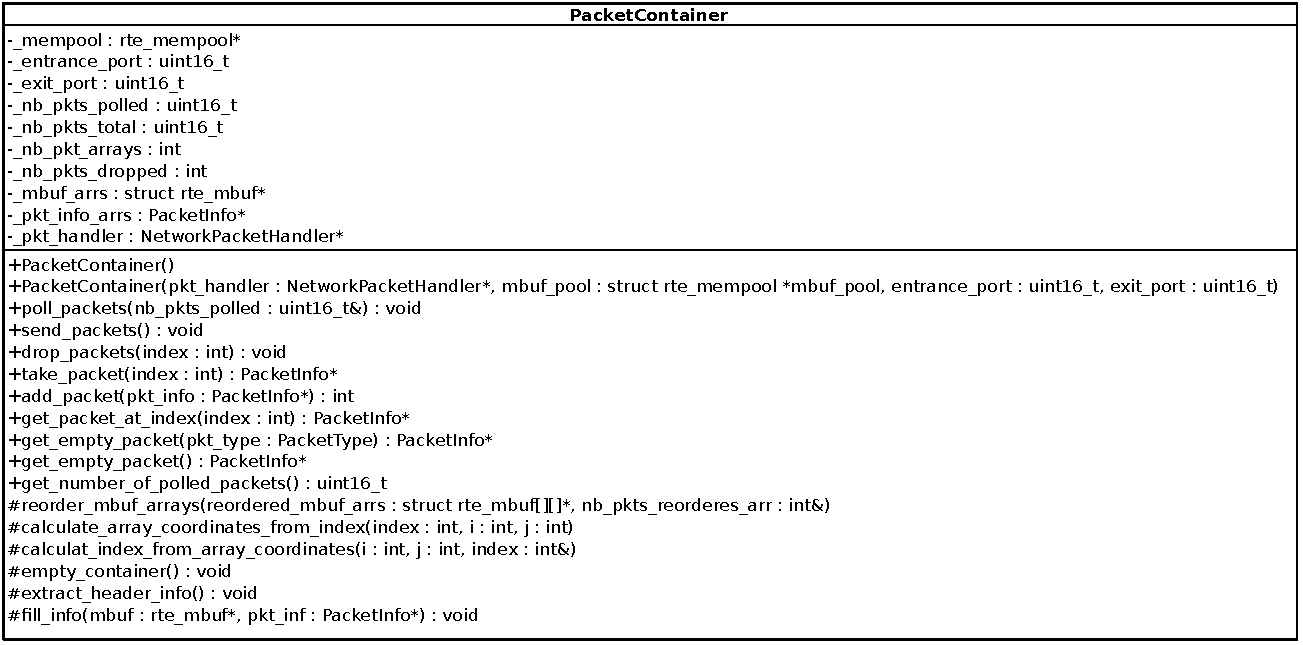
\includegraphics[width=\linewidth]{img/PacketContainerClass.pdf}
    \caption{Klassendiagramm PacketContainer}
    \label{Klassendiagramm_PacketContainer}
\end{figure}

Der \texttt{PacketContainer} ist keine aktive Klasse und wird aufgerufen, um spezielle, im Abb. \ref{Klassendiagramm_PacketContainer} angegebene, Aufgaben umzusetzen. Eine dieser Aufgaben ist das Polling von Paketen, dessen Ablauf im Sequenzdiagramm \ref{Sequenzdiagramm_PacketDissection} dargestellt wird. Eine weitere Aufgabe ist das Verwerfen von Paketen, welches durch \texttt{drop\_packet(int index)} umgesetzt wird. Hierbei wird dem \texttt{NetworkPacketHandler} mitgeteilt, welcher \texttt{mbuf} verworfen werden soll und die Referenzen im \texttt{PacketContainer} selbst gelöscht.

Es ist aber auch möglich, mittels der Methode \texttt{take\_packet(int Index):PacketInfo*} Pakete aus dem \texttt{PacketContainer} zu entfernen, ohne sie zu löschen. Dafür werden nur die\\ \texttt{PacketContainer}-internen Referenzen auf den \texttt{mbuf} und seine \texttt{PacketInfo} zu Nullreferenzen gesetzt und die \texttt{PacketInfo} zurückgegeben. Diese entnommenen Pakete können später wieder mit \texttt{add\_packet(PacketInfo* pkt\_info):int} eingefügt werden. Dafür wird dieses Paket hinter den bereits existenten Pakete im \texttt{mbuf}-Array gespeichert. Selbiges wird für die zugehörige \texttt{PacketInfo} gemacht. Zurückgegeben wird der Index, unter dem das neue Paket zukünftig erreichbar sein wird. Es können nicht nur zuvor entnommene Pakete einem \texttt{PacketContainer} hinzugefügt werden, sondern auch komplett neue. Dieses Erstellen von Paketen ist mit dem Befehl \texttt{get\_empty\_packet(PacketType pkt\_type):PacketInfo*} möglich. Hierbei wird für einen neuen \texttt{mbuf} Speicher aus einem \texttt{mempool} alloziert und eine zugehörige \texttt{PacketInfo} vom gewünschten \texttt{PacketType} erstellt. Mithilfe dieser \texttt{PacketInfo}, kann der Paketkopf im Anschluss befüllt werden. Zuletzt müssen all diese Pakete auch wieder mit \texttt{send\_packets()} versendet werden. Dafür wird das \texttt{mbuf}-Array, falls notwendig, umsortiert, da durch \texttt{drop\_packet(int index)} Lücken entstehen können und DPDK nicht mit Nullreferenzen umgehen kann. Zuletzt wird das Array über den NetworkPacketHandler an DPDK zur Versendung übergeben.

Auch wenn bisher immer nur von je einem Array für \texttt{mbuf}s und \texttt{PacketInfos} gesprochen wurde, können es mehrere werden. Es gibt bei DPDK eine sogenannte BurstSize, welche angibt, wie viel Pakete maximal auf einmal entgegengenommen und wieder versendet werden können. Daran sind auch die Größen der Arrays angepasst. Da es aber durch Maßnahmen des \texttt{Treatments} und \texttt{Inspection} zur Erzeugung von neuen Paketen kommen kann, gibt es zusätzliche Arrays, falls die ersten bereits voll sind. Die Verwaltung dieser Arrays ist in allen Funktionen enthalten und hat nach außen keinen sichtbaren Effekt.

\subsection{PacketInfo}
Die genaue Umsetzung, sowie die daraus resultierende Befüllung hat sich im Laufe der Entwicklungsphase sehr stark verändert. Dies hatte vor allem Performance-Gründe. In der aktuellen Variante ist die \texttt{PacketInfo} selbst nur für die Verwaltung des \texttt{mbuf}s sowie das Speichern seines Layer 3 und 4-Protokolls verantwortlich.

Um ausschließlich notwendige Informationen zu speichern, wird diese \texttt{PacketInfo} in eine protokollspezifische Variante gecastet. Diese spezialisierten Varianten erben von der eigentlichen \texttt{PacketInfo} und erweitern sie um Getter- und Setterfunktionen für die relevanten Header-Informationen ihrer jeweiligen Protokolle.

Auch wenn in Diagramm \ref{Klassendiagramm_PacketInfo} \texttt{PacketInfos} mit IPv6 aufgeführt werden, sind diese noch nicht funktionsfähig. Es wurde sich entsprechend der Anforderungen zuerst auf IPv4 konzentriert.

\begin{figure}
    \centering
    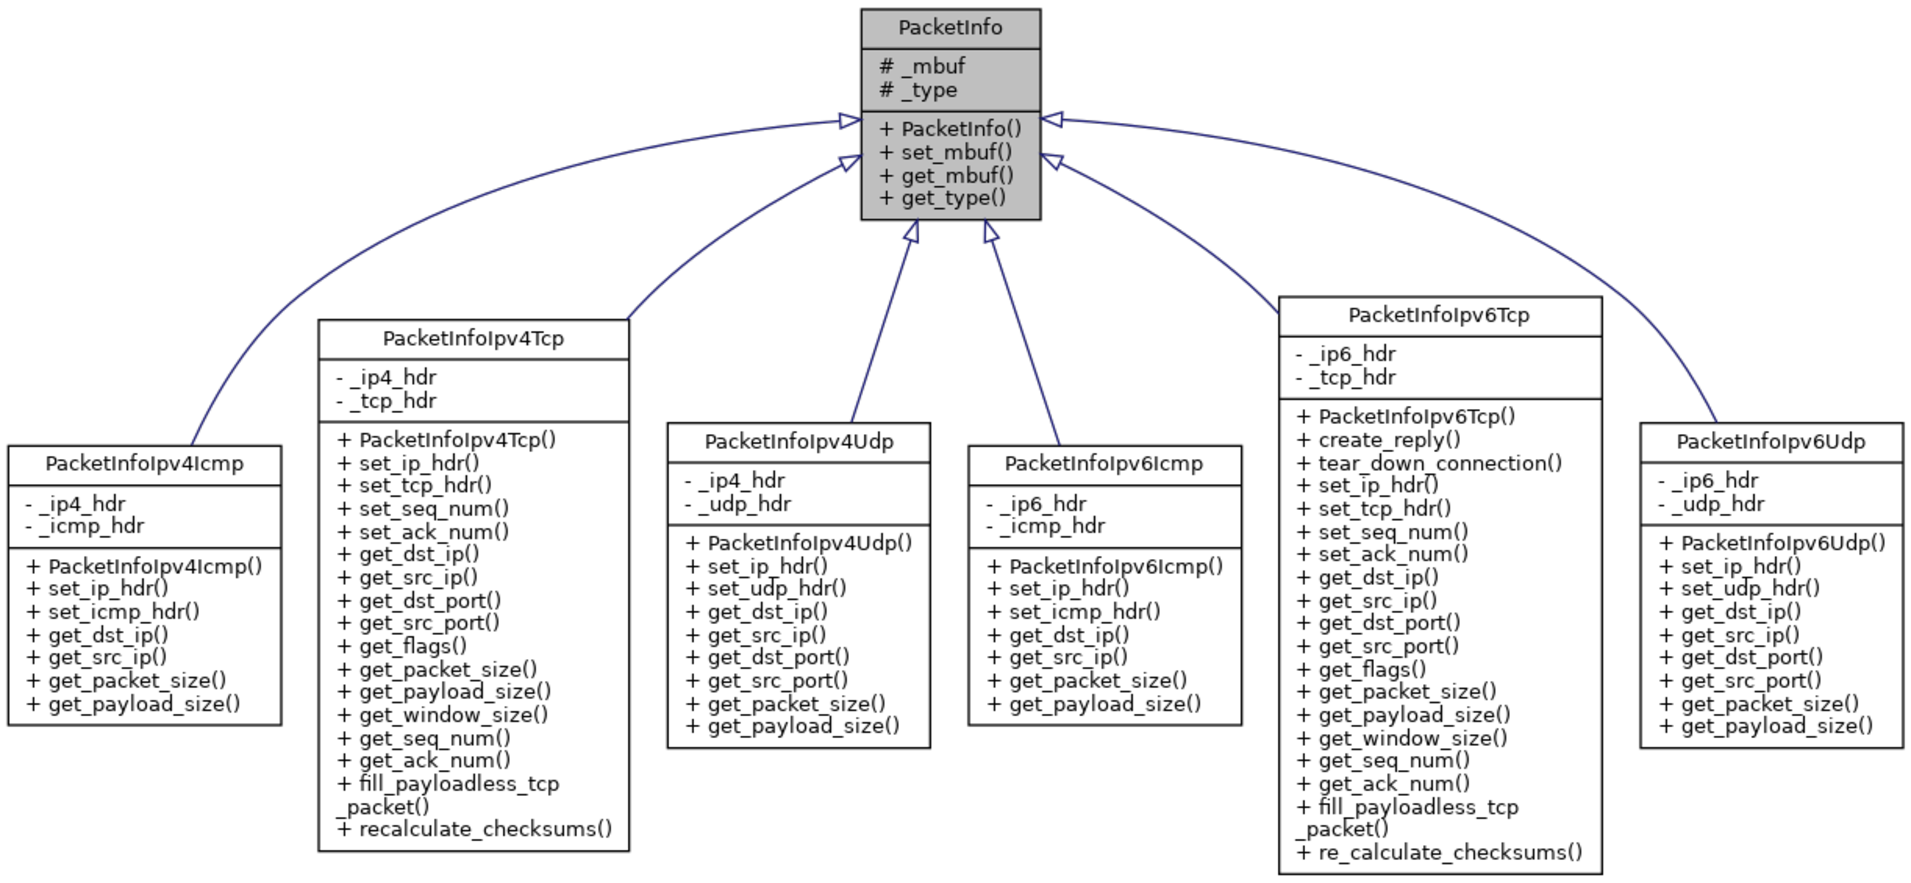
\includegraphics[width=\linewidth]{img/PacketInfoInheritance.pdf}
    \caption{Klassendiagramm aller PacketInfo Varianten}
    \label{Klassendiagramm_PacketInfo}
\end{figure}

\subsection{HeaderExtractor}
Wie bereits erwähnt, wurde die Extraktion der Headerinformationen dezentralisiert und wird nur bei Abruf entsprechender Informationen durchgeführt. Dies führte zu einer Verringerung von Code für den \texttt{HeaderExtractor} im Laufe der Entwicklung, weshalb er in den \texttt{PacketContainer} integriert wurde. In obigen Sequenzdiagramm stellt er die Funktionen \texttt{extract\_header\_info()} und \texttt{fill\_info(rte\_mbuf* mbuf, PacketInfo* pkt\_inf)}.

Dabei wird in \texttt{extract\_header\_info()} über die einzelnen Elemente des \texttt{PacketContainers} iteriert und für jeden \texttt{mbuf} die Funktion \texttt{fill\_info(rte\_mbuf* mbuf, PacketInfo* pkt\_inf)} aufgerufen, welche wiederum den \texttt{PacketInfoCreator} ausführt und den \texttt{mbuf} mit der zugehörigen \texttt{PacketInfo} verknüpft.

\subsection{PacketInfoCreator}
Diese Klasse ist ein Hilfsmittel, um Vererbungsketten zu vermeiden. Ihre Aufgabe ist es, die zum Paket passende \texttt{PacketInfo}-Version zu erzeugen. Dabei liest der \texttt{PacketInfoCreator} die Layer 3 und Layer 4-Protokoll-IDs aus, legt die entsprechenden \texttt{structs} auf den Speicher und speichert sie in der frisch erzeugten \texttt{PacketInfo}.

\section{Inspection}
Die \texttt{Inspection} ist für die Erkennung böswilliger IP Pakete zuständig und untersucht diese daher auf verdächtige Strukturen und Muster. Dazu wird auch eine eigene lokale Statistik erstellt, zur Auswertung genutzt und zur Informationsweitergabe mit einer globalen Statistik geteilt.

Der \texttt{Initializer} erstellt für jeden genutzten Thread eine eigene Inspektion, welche alle Pakete dieses Threads analysiert und DDoS-Attacken erkennt. Dazu wird der \texttt{Inspection} jeweils ein \texttt{PacketContainer} übergeben, der eine Menge von Paketen enthält, die über das \texttt{NicManagement} eingegangen sind.

Die Erkennung basiert auf einer Mustererkennung von zeitlich aufeinanderfolgenden Paketen nach einer Auftrennung in die Protokolle UDP, TCP und ICMP. UDP und ICMP Pakete werden ausschließlich mit einem vorher festgelegten Threshold geprüft, der sich an eine selbst berechnete Angriffsrate anpasst. TCP Pakete werden zusätzlich auf Zero und Small Window sowie auf SYN-FIN und SYN-FIN-ACK Muster überprüft.

Der Ablauf und Reihenfolge der Prüfungen der \texttt{Inspection} ist aus einer Versuchsdurchführung mit einem Decision Tree für DDoS-Abwehr entstanden, um einen möglichst schnellen und effizienten Ablauf zu finden. Implementiert wurde eine statische, nicht veränderliche Pipeline, die nach den größten auszuschließenden Faktoren jedes Pakets vorgeht.

Der Ablauf kann grob in drei Filterstufen, auch Security Layers genannt, unterteilt werden:
\begin{enumerate}
    \item RFC Compliance
    \item Static Rules
    \item Dynamic Rules
\end{enumerate}
Ob ein Paket dem RFC Standard entspricht, wird bereits bei der \texttt{PacketInfo} klar. Die Klasse \texttt{Inspection} bietet die Möglichkeit, bestimmte Fehler zuzulassen oder Pakete mit bestimmten Fehlern zu blockieren und zu löschen.

Die zweite Stufe der Filter setzt sich aus fest definierten Angriffen und Angriffsmustern zusammen. So sind zum Beispiel bei SYN-FIN und SYN-FIN-ACK Angriffen immer die Flags SYN und FIN oder SYN, FIN und ACK gesetzt. So können diese sofort erkannt und das Paket verworfen werden. Weitere Angriffe, die in der statischen Abwehr erkannt werden, sind Zero- und Small-Window Angriffe.

\begin{figure}[H]
    \centering
    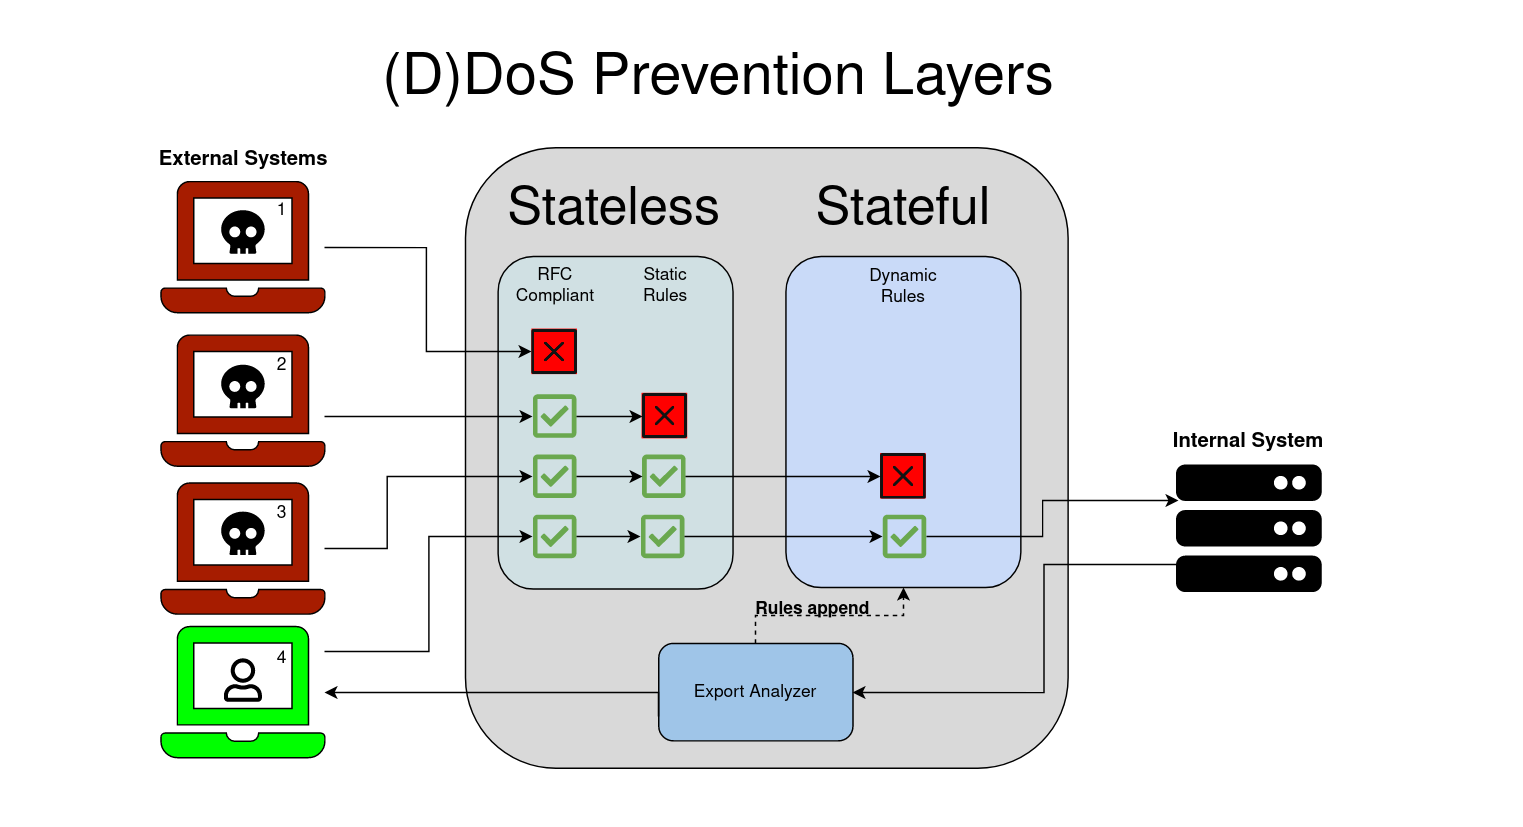
\includegraphics[width=\linewidth]{img/Security_Layers.png}
    \caption{Stufen der Sicherheit}
    \label{security_layers}
\end{figure}

In der dynamischen Filterstufe werden die Filterregeln entsprechend dem aktuellen Netzwerkverkehr und vorher eingegangenen Paketen angepasst. So dient ein Limit der Paketrate (engl. Threshold) dazu, UDP und TCP Floods abzuwehren. Eigene Verbindungstabellen der ausgehenden Netzwerkverbindungen lassen jedoch legitime Pakete, die als Antwort auf eine bestehende Verbindung dienen, weiterhin zu, um den legitimen Netzwerkverkehr nicht einzuschränken.

Die Verknüpfung und Ablauf der Filterung wird in der Abbildung. \ref{security_layers} vereinfacht dargestellt.

Im Diagramm \ref{security_layers} muss Folgendes unterschieden werden: Die Computer 1 bis 3 sind Angreifer mit unterschiedlichen Angriffen, die ebenso in unterschiedlichen Filterstufen als Angriff erkannt werden und Computer 4 als Nutzer mit legitimen Anfragen an den Server, die den Filterregeln entsprechen.
Ausgehender Verkehr aus dem internen System wird grundsätzlich vertraut und nicht zusätzlich gefiltert. Jedoch wird ausgehender Verkehr analysiert, um die dynamischen Regeln anzupassen.

Nach jedem Durchlauf eines \texttt{PacketContainer}s werden die lokalen und globalen Statistiken aktualisiert. Die Weitergabe der Informationen an die Statistik erfolgt über einen eigenen Interthread- Kommunikationskanal zum globalen Statistik-Thread. Die globale Statistik führt alle einzelnen Informationen zusammen und macht sie dem Nutzer in einfacher Weise abrufbar.
\begin{figure}[h]
    \centering
    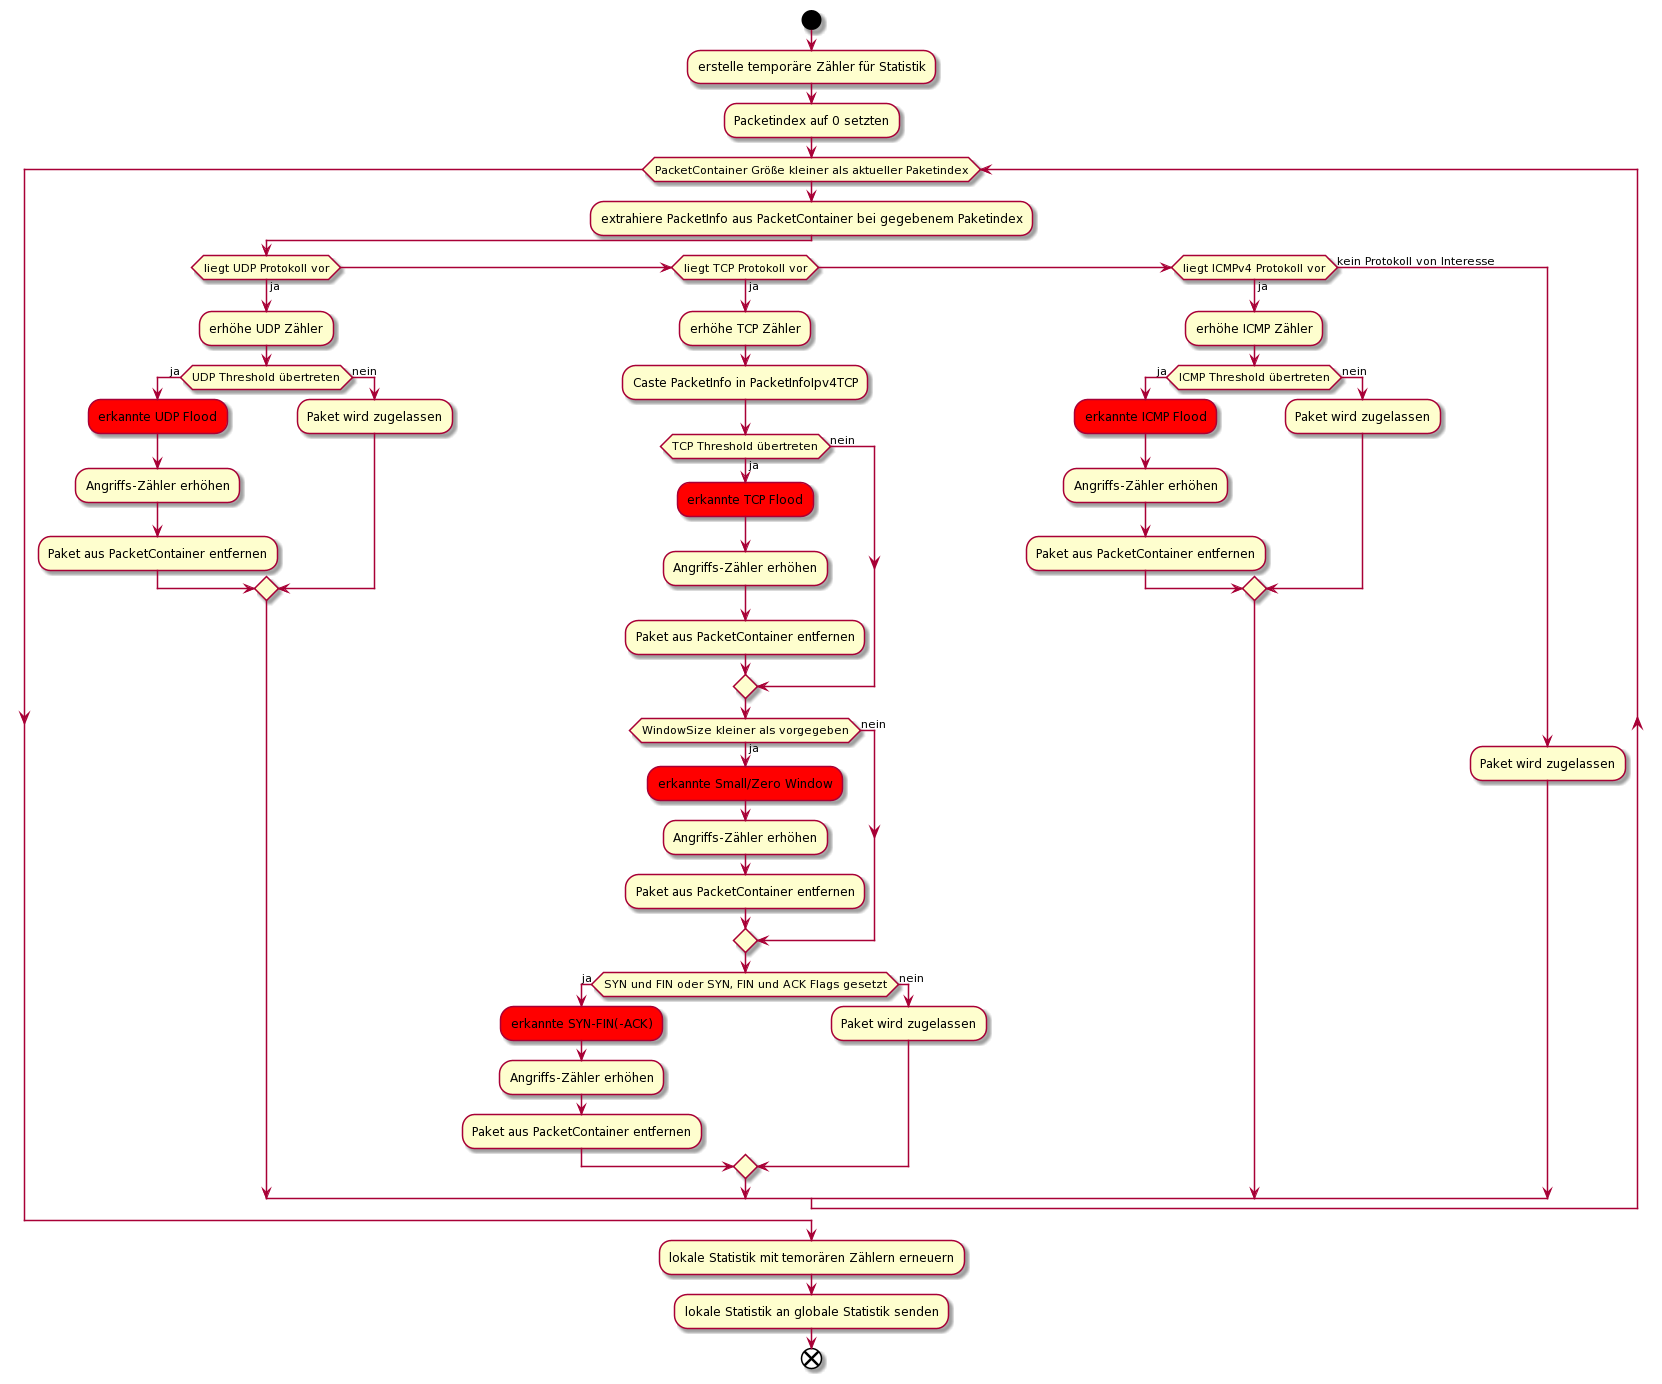
\includegraphics[angle=270, width=\linewidth]{img/inspection_ablauf.png}
    \caption{Aktivitätsdiagramm der Methode \texttt{analyzeContainer()} der Inspection}
    \label{inspection_activity}
\end{figure}

\section{Treatment}
Das \texttt{Treatment}, welches für die Behandlung der SYN-Flut zuständig ist, erhält vom \texttt{Thread} zwei Pointer auf \texttt{PacketContainer}. Für jede Senderichtung, sowohl von Intern nach Extern als auch umgekehrt, existiert einer dieser Container. Der Ablauf in der Behandlung von Paketen unterscheidet sich basierend auf deren Senderichtung. Jedes Paket wird im \texttt{Treatment} zwar einzeln, allerdings im Kontext der gesamten Verbindung betrachtet. Die Behandlung im \texttt{Treatment} beginnt mit dem Iterieren über die Einträge im jeweiligen \texttt{PacketContainer}. Hierbei wird zugleich geprüft, ob das gerade betrachtete Paket bereits gelöscht wurde, oder von einem Typ ist, welcher nicht im \texttt{Treatment} behandelt wird. Dies ist auch im globalen Ablauf der Funktion \texttt{treat\_packets()} in Abbildung \ref{Aktivität_treat_packet_0} sowie \ref{Aktivität_treat_packet_1} zu erkennen. Sollte dies der Fall sein, wird ebendieser Eintrag übersprungen. Sollte es sich bei dem gerade betrachteten Paket beispielsweise um ein UDP-Paket handeln, so wird dieses im Treatment nicht weiter betrachtet, da dies bereits in der \texttt{Inspection} geschah.

Nach diesen ersten Tests findet jeweils eine Fallunterscheidung statt. Für Pakete, welche von extern nach intern geschickt werden sollen, gilt:

Falls es sich bei dem Paket um ein TCP-SYN-Paket handelt, so wird als Antwort hierauf ein SYN-ACK generiert, dessen Sequenznummer durch einen, vom Programm berechneten, SYN-Cookie ersetzt wird. Hierzu existiert die Methode \texttt{calc\_cookie\_hash()}, welche 24 der 32 Bit langen Sequenznummer generiert, welche später mit einem 8 Bit Zeitpunkt (engl. \glqq Timestamp\grqq) in der Methode \texttt{treat\_packets()} aufgefüllt werden. Dieser SYN-Cookie enthält Informationen über die Verbindungsentitäten, sowie zur Verbesserung der Effektivität einen Zeitstempel und ein Secret. Dieser SYN-Cookie ermöglicht es, im Verlauf des Verbindungsaufbaus auf das Speichern von Informationen über die Verbindung zu verzichten. Somit wird die Angriffsfläche von SYN-Floods effektiv minimiert.

Sollte ein ACK als Reaktion auf dieses SYN-ACK erhalten werden, so ist durch die Funktion \texttt{check\_syn\_cookie()} zu überprüfen, ob der empfangene Cookie in Form der Sequenznummer plausibel ist (Siehe Abb. \ref{check_syn_cookie}). Das bedeutet, dass der Zeitstempel maximal eine Zeiteinheit alt ist, welche in diesem Programm 64 Sekunden dauert, und der restliche Cookie mit dem erwarteten Cookie übereinstimmt. Der Cookie setzt sich insgesamt zusammen aus 8 Bit Timestamp, sowie 24 Bit Hashwert über externe und interne IP-Adresse, externe und interne Portnummer sowie dem Timestamp und dem Cookie\_Secret.
Des weiteren ist eine Verbindung mit dem internen Server, spezifiziert in der DestIP des ACK-Paketes, aufzubauen. Zudem muss die dem ACK hinzugefügten Payload gespeichert werden, auch dies geschieht in einer separaten Map, der ACKmap. Dieses ACK-Paket muss nach erfolgreichem Verbindungsaufbau mit dem internen Server an ebendiesen verschickt werden.

Wird ein SYN-ACK von extern empfangen, so ist dies ohne Veränderung an das interne Netz zuzustellen. Allerdings muss hier ein Eintrag in der Offsetmap erzeugt werden, wobei der Offset realisierungsbedingt null ist.

Werden Pakete ohne gesetzte Flags, beziehungsweise nur mit gesetztem ACK-Flag verschickt, so findet eine Sequenznummernzuordnung und eine Anpassung von Sequenznummern statt. Hierzu wird eine Densemap mit individueller Hashfunktion, in diesem Fall XXH3, verwendet. Bei der Densemap handelt es sich um eine besonders effiziente Hashmap, welche ein Einfügen, Suchen und Löschen in bis zu vier mal weniger Zeit als eine unordered\_map ermöglicht. Die Auswahl der Hashfunktion XXH3 ist  dadurch motiviert, dass sie extrem schnell ist und dennoch kaum Kollisionen erzeugt. Insbesondere werden durch sie bereits auf handelsüblichen Computersystemen Hashraten von bis zu 31.5 Gbit/s erzielt.

Der Ablauf beim Empfang eines solchen Paketes ist wie folgt: Bei eingehenden Paketen wird ein zuvor berechneter Offset, welcher in der Offsetmap für jede Verbindung gespeichert ist, von der ACK-Nummer subtrahiert.

Wird ein ACK empfangen, welches zu einer Verbindung gehört, in deren Info finseen auf true gesetzt ist, so muss die ACK-Nummer angepasst, das Paket an den internen Server geschickt und der Eintrag in der Densemap verworfen werden.

Falls ein Paket mit gesetztem RST-Flag von extern empfangen wird, wird der Eintrag in der Densemap gelöscht und das empfangene Paket an den internen Server weitergeleitet. Hierbei muss keine Anpassung der ACK-Nummer vorgenommen werden.

Sollte ein FIN empfangen werden, so muss im Info-Struct, welches Teil der Offsetmap ist, der Wert finseen auf true gesetzt werden. In diesem Fall ist das Paket nach Anpassung der ACK-Nummer weiterzuleiten.

Im zweiten Fall der übergeordneten Fallunterscheidung erhält das Programm anschließend den \texttt{PacketContainer} der Pakete, welche das Netz von intern nach extern verlassen wollen. Auch hier wird, bevor ein Paket der Behandlung unterzogen wird, geprüft, ob das Paket nicht bereits gelöscht wurde oder es sich um ein Paket falschen Typs handelt.

Erhält das System ein SYN-Paket von einem internen Server, so wird dieses an das im Paket spezifizierte Ziel weitergeleitet. Eine Anpassung der Sequenznummer findet in diesem Fall nicht statt.

Erhält das System ein SYN-ACK aus dem internen Netz, so muss das System die Differenz aus der ACK-Nummer dieses Pakets. und der des in der ACKmap gespeicherten Paketes berechnen. Dieser Wert wird als Offset in der Offsetmap eintragen. Das von intern empfangene SYN-ACK Paket muss verworfen werden.
Das zuvor in der ACKmap zwischengespeicherte Paket muss nun mit angepasster ACK-Nummer intACK = extACK-offset an den internen Host geschickt werden.

Wird ein Paket ohne gesetzte Flags oder mit gesetztem ACK-Flag von Intern nach Extern verschickt, so findet eine weitere Fallunterscheidung statt.
Im Fall, dass finseen bereits auf true gesetzt ist, muss der Offset in der Offsetmap nachgeschlagen werden, der Eintrag daraufhin gelöscht werden und das empfangene Paket mit extSeq = intSeq + offset verschickt werden.
Gesetzt den Fall, dass noch kein Eintrag in der Offsetmap existiert, muss ein neuer Eintrag in dieser erstellt werden. Der Offsetwert muss auf null, und finseen auf false gesetzt werden. Das empfangene Paket muss hiernach nach Intern weitergeleitet werden.
Trifft keiner der beiden obigen Fälle ein, so muss der Offset in der Offsetmap nachgeschlagen werden und das empfangene Paket nach Intern weitergeschickt werden. Vor dem Versenden muss hierbei die Sequenznummer wie folgt angepasst werden: extSeq = intSeq + offset.

Sollte ein Paket mit gesetztem FIN-Flag erkannt werden, so ist diese Information in der Info an Stelle Key = Hash(extip, intip, extport, intport) mit dem Vermerk finseen = true, zu speichern. Das empfangene Paket ist durch das System nach extern mit extSeq = intSeq + offset weiterzuschicken.

Wird ein RST erhalten, so ist eine Anpassung der Sequenznummer vorzunehmen, das Paket entsprechend weiterzuleiten und der Eintrag in der Offsetmap an entsprechender Stelle zu entfernen.

Des weiteren könnte es unter Umständen erforderlich werden, die Einträge mit einem Timestamp zu versehen, welcher speichert, wann dieser Eintrag zuletzt verwendet wurde, sollte es zu Situationen kommen, in denen sowohl Sender als auch Empfänger die Verbindung nicht korrekt terminieren können. Dies ist bisweilen nicht implementiert, die Idee wird allerdings basierend auf den Ausgängen der Tests auf dem Testbed weiter verfolgt oder verworfen.

\begin{figure}[h]
    \centering
    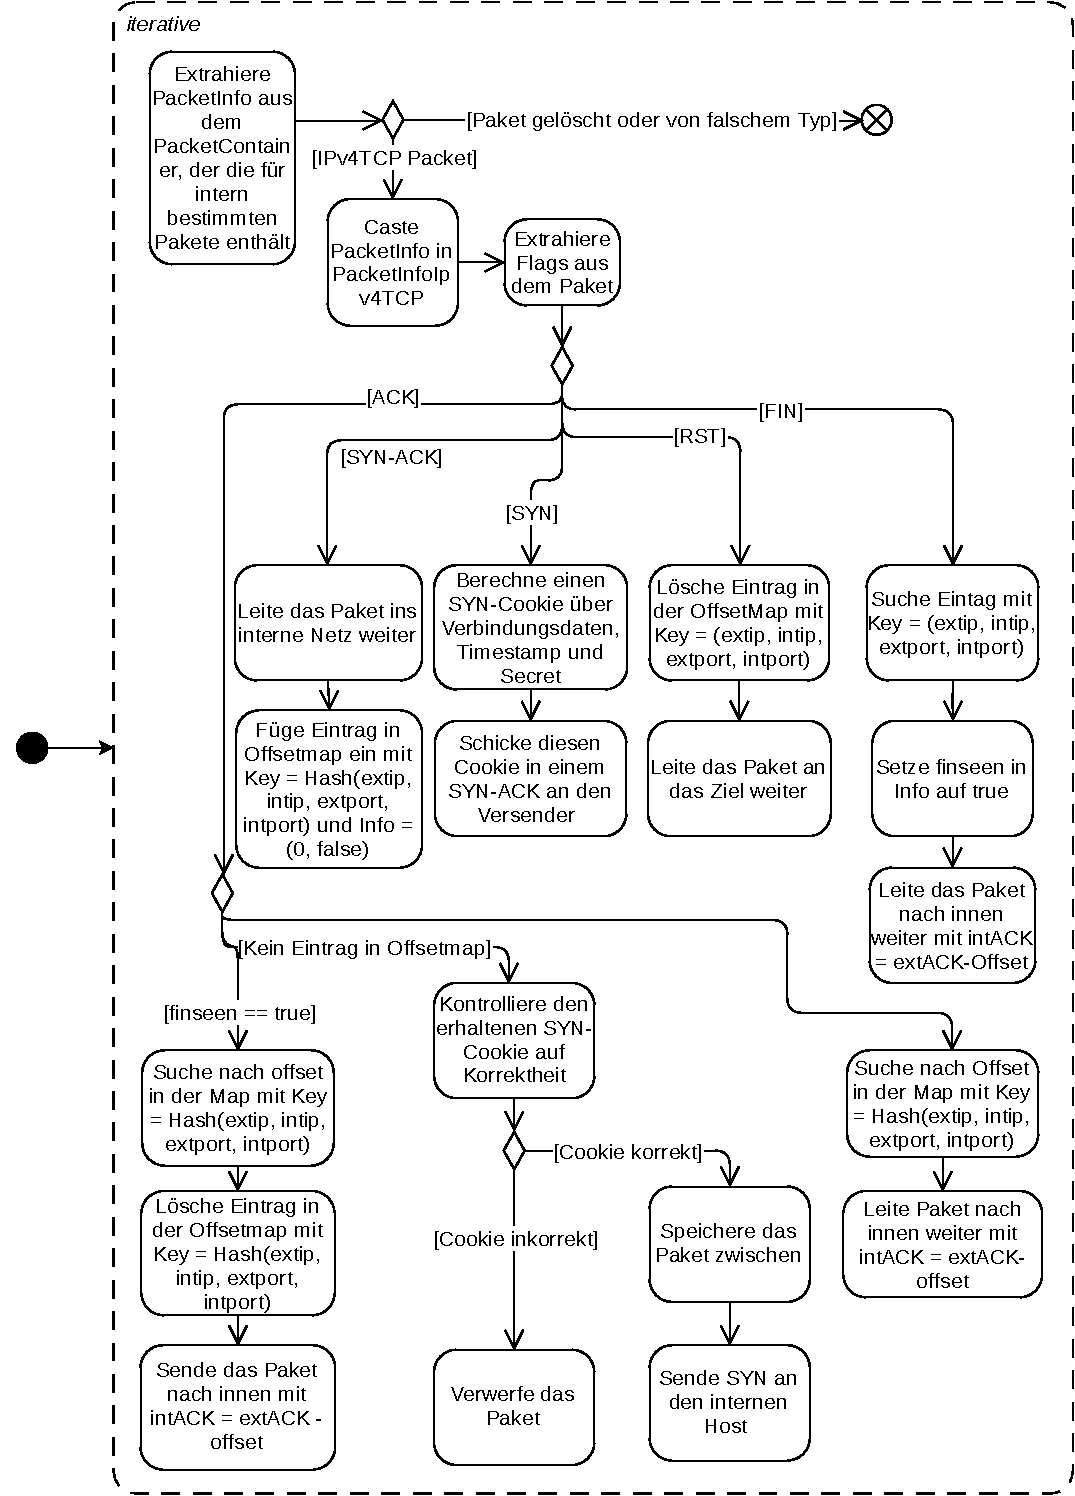
\includegraphics[width=0.98\linewidth]{img/treat_packets_0.pdf}
    \caption{Aktivitätsdiagramm der Methode \texttt{treat\_packets()}, Teil: Pakete nach Intern}
    \label{Aktivität_treat_packet_0}
\end{figure}
\begin{figure}[h]
    \centering
    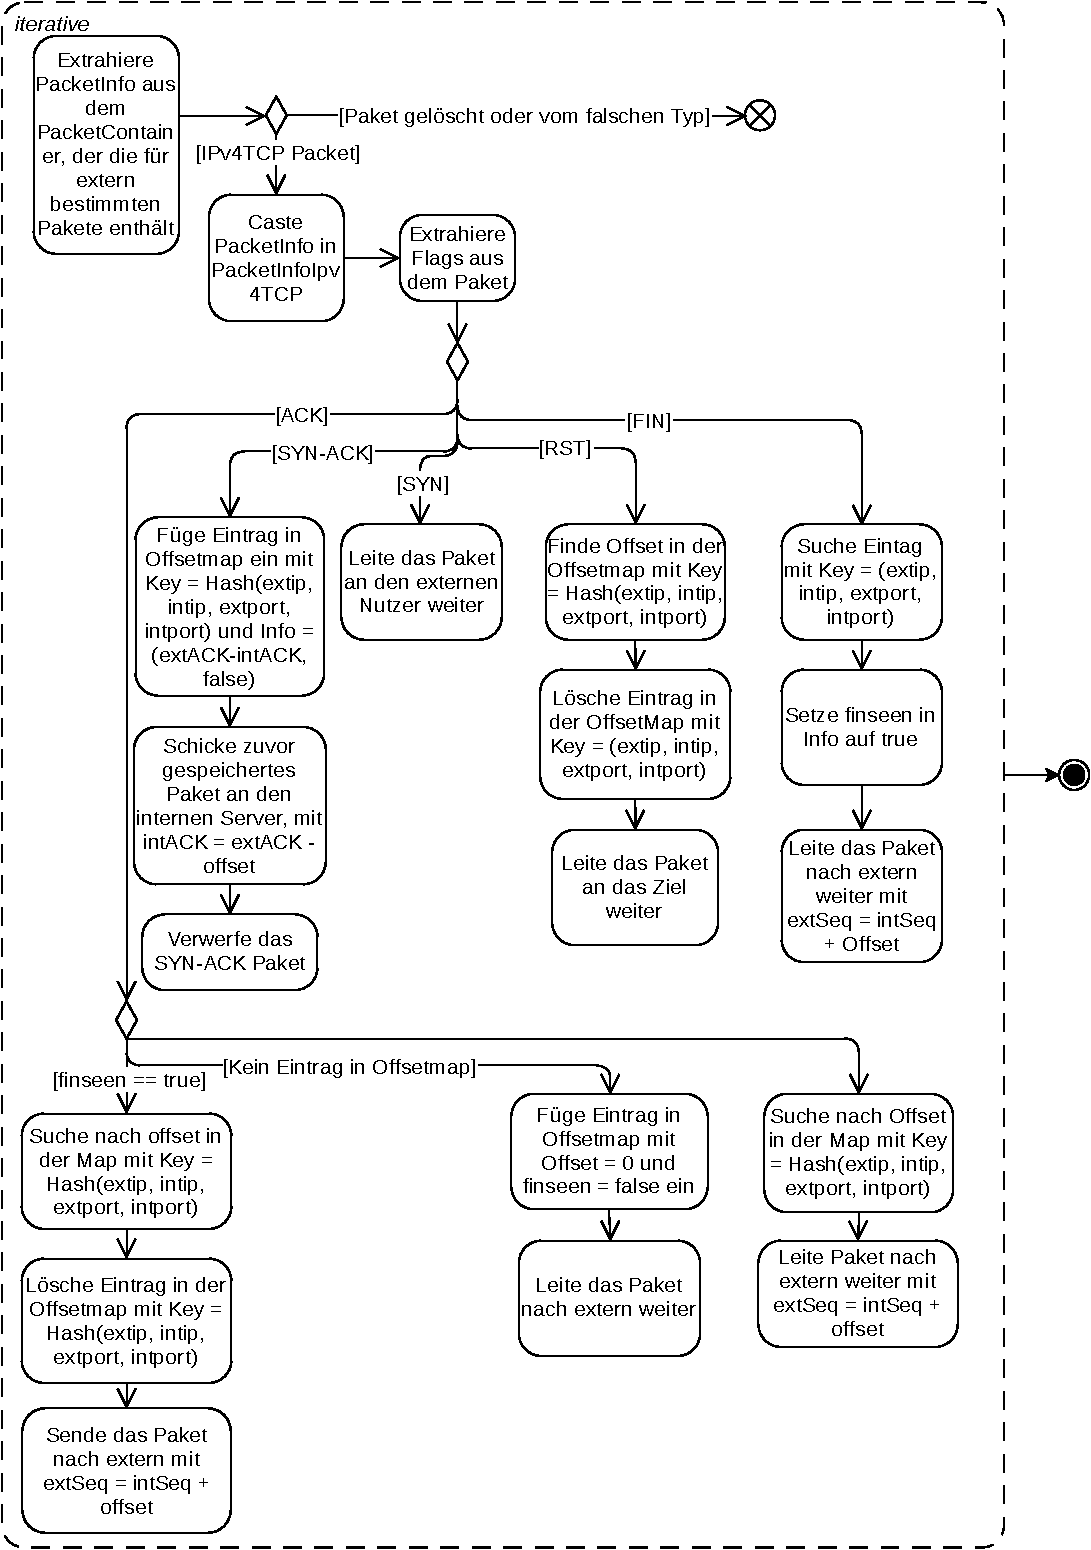
\includegraphics[width=0.96\linewidth]{img/treat_packets_1.pdf}
    \caption{Aktivitätsdiagramm der Methode \texttt{treat\_packets()}, Teil: Pakete nach Extern}
    \label{Aktivität_treat_packet_1}
\end{figure}

\begin{figure}[t]
    \centering
    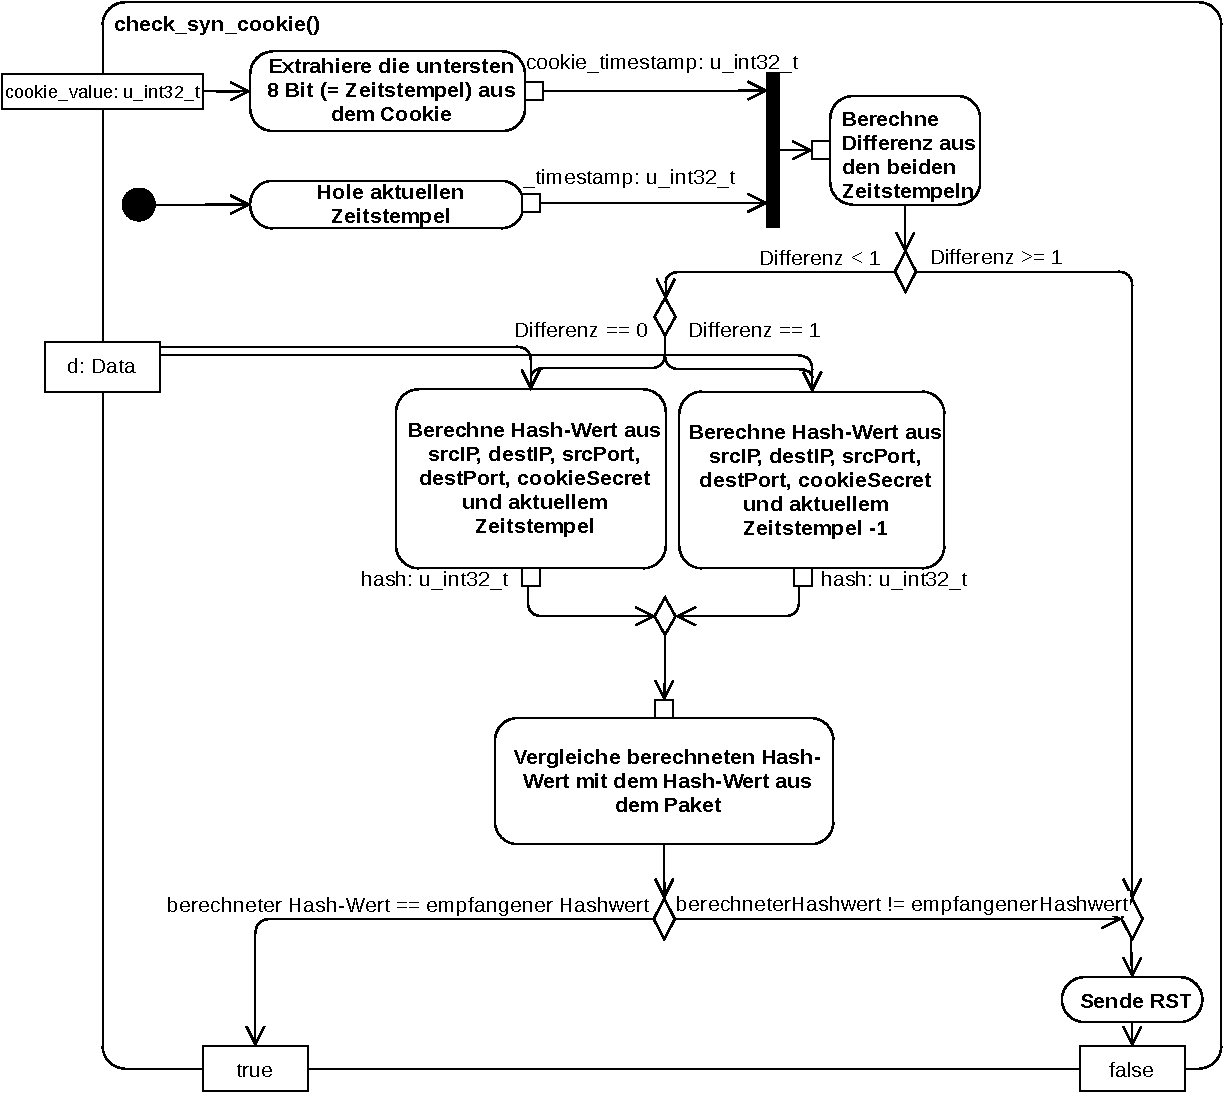
\includegraphics[width=\linewidth]{img/check_typ_syn_cookie_neu.pdf}
    \caption{Aktivitätsdiagramm der Methode \texttt{check\_syn\_cookie()}}
    \label{check_syn_cookie}
\end{figure}
Nachdem ein ACK als Reaktion auf ein SYN-ACK bei dem zu entwerfenden System angekommen ist, wird die Methode \texttt{check\_typ\_syn\_cookie()} aufgerufen.
Grundsätzlich wird hier überprüft, ob der Hash-Wert aus dem empfangenen Paket mit dem eigens berechneten Hash-Wert übereinstimmt. Falls dies nicht der Fall ist oder die Differenz der Zeitstempel zu groß ist, wird ein Paket mit gesetzten Reset-Flag (RST) an den Sender geschickt. Dieses Flag zeigt an, dass die Verbindung beendet werden soll. Andernfalls wird die Verbindung als legitim erkannt und das Paket in der ACKmap zwischengespeichert bis die Verbindung mit dem internen System erfolgreich war.

Abbildung \ref{createcookiesecret} zeigt die parameterlose Methode \texttt{create\_cookie\_secret()}. Zu Beginn werden drei 16 Bit lange Zufallszahlen generiert, wobei auf die Funktion \texttt{rand()} aus der C Standardbibliothek zugegriffen wird. Der erste mit \texttt{rand()} generierte Wert wird um 48 Bit nach links verschoben, der zweite um 32 Bit. Diese beiden Werte werden danach bitweise ODER miteinander verknüpft. Dieser verknüpfte Wert wird dann wiederum mit der dritten zufälligen 16 Bit Zahl bitweise ODER verknüpft. Das Ergebnis dieser Verknüpfung ist eine 64 Bit lange Zufallszahl, die von der Methode zurückgegeben wird.

\begin{figure}[H]
    \centering
    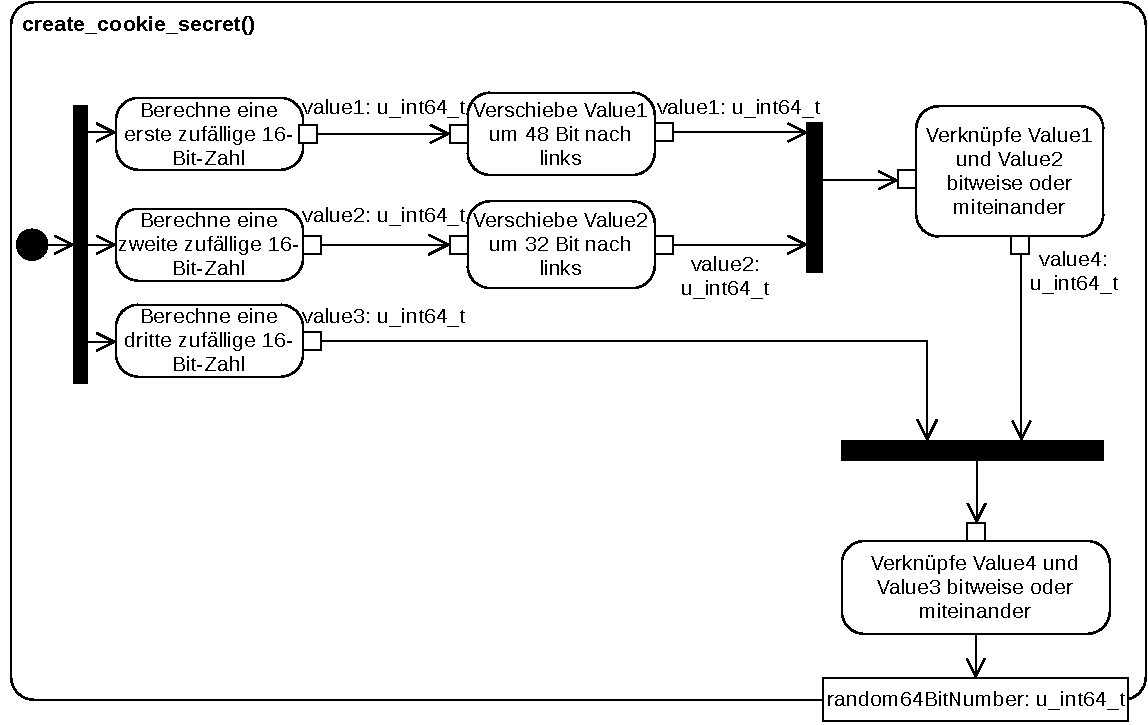
\includegraphics[width=\linewidth]{img/create_cookie_secret_neu.pdf}
    \caption{Aktivitätsdiagramm der Methode \texttt{create\_cookie\_secret()}}
    \label{createcookiesecret}
\end{figure}

\end{document}
